\documentclass{beamer}

\usepackage{graphicx,hyperref,udesc,url}
\usepackage[utf8]{inputenc}
\usepackage[T1]{fontenc}
\usepackage[portuges]{babel}
\usepackage{booktabs}
\usepackage{caption}
\usepackage{subcaption}
\usepackage{amssymb}
\usepackage{multirow}
\usepackage{colortbl}

\setbeamertemplate{caption}[numbered]

\newcommand{\RNum}[1]{\uppercase\expandafter{\romannumeral #1\relax}}

\AtBeginSection[]{
    \begin{frame}
    \vfill
    \centering
    \begin{beamercolorbox}[sep=8pt,center,shadow=true,rounded=true]{title}
        \usebeamerfont{title}\insertsectionhead\par%
    \end{beamercolorbox}
    \vfill
    \end{frame}
}

\usepackage[
    backend=bibtex,
    style=alphabetic,
    citestyle=authoryear
]{biblatex}

\addbibresource{bibliografia.bib}

\newcommand{\ccite}[1]{(\citeauthor{#1}, \citeyear{#1})}

\title[]{Proposta de um algoritmo híbrido para a solução do Problema de Escalonamento de Tripulação}

\author[Renan S. Silva]{
    Renan S. Silva\\\medskip
    {\small \url{uber.renan@gmail.com}} \\ 
}

\institute[UDESC]{
    Departamento de Ci\^encia da Computa\c{c}\~ao \\
    Centro de Ci\^encias e Tecnol\'ogias\\
    Universidade do Estado de Santa Catarina
}

\begin{document}

\begin{frame}
    \titlepage

\end{frame}

\begin{frame}{Overview}
    \tableofcontents
\end{frame}

\section{Introdução}
\begin{frame}
    \frametitle{Introdução}

    \begin{figure}[!htb]
        \centering
        \begin{minipage}{0.48\textwidth}
            \begin{itemize}
                %\item Segundo~\ccite{de2011algoritmo} e~\ccite{qiao2010algorithm}, o planejamento operacional de uma empresa de transporte de urbano pode ser dividido conforme a figura~\ref{fig_etapas};
                \item O planejamento operacional de uma empresa de transporte de urbano pode ser dividido conforme a figura~\ref{fig_etapas};
                \item Este trabalho tem como objetivo propor um algoritmo para resolver problema do Escalonamento de Tripulação (CSP);
            \end{itemize}
        \end{minipage}
    %
        \begin{minipage}{.48\textwidth}
        {
            \centering
            \includegraphics[height=0.8\textheight]{../tcc/figuras/etapas.pdf}
            \captionof{figure}{Etapas do planejamento}
            \label{fig_etapas}
        }
        \end{minipage}
    \end{figure}
\end{frame}

\begin{frame}
    \frametitle{Relevância}

    \begin{description}
        \item [Teória] O CSP é um problema $\mathcal{NP}$-Hard, que pode ser reduzido para o problema de cobertura ou particionamento de conjuntos;
        \item [Prática]\ccite{zeren2012improved} afirma que os gastos com a tripulação são a segunda maior fonte de gastos das empresas, atrás apenas dos gastos com combustíveis;
    \end{description}
\end{frame}

\begin{frame}
    \frametitle{Definição}

    O CSP consiste determinar jornadas para um conjunto de tripulantes, onde

    \begin{description}
        \item[Tarefa] É uma atividade que deve ser realizada, que possui um tempo de inicio e fim predefinidos;
        \item[Jornada] É um conjunto de tarefas que devem ser executadas por uma mesma tripulação;
        \item[$\blacktriangleright$]Jornadas possuem restrições, carga horaria máxima, etc;
        \item[$\blacktriangleright$]Existe um custo para deslocar-se entre duas tarefas;
        \item[$\blacktriangleright$]Deseja-se minimizar o custo total de cobrir todas as jornadas;
    \end{description}
\end{frame}

\section{Formulação}
\begin{frame}
    \frametitle{Problema de cobertura e particionamento}
    Dentre as possíveis modelagens possíveis para o CSP, utilizou-se uma com base no problema de particionamento de conjuntos(SPP);

    \begin{figure}[!htb]
        \centering
        \begin{minipage}{0.48\textwidth}
            $A = \begin{pmatrix}
                1 & 1 & 0 & 0 & 0 & 0 & 0 \\
                0 & 0 & 1 & 1 & 1 & 1 & 1 \\
                1 & 0 & 1 & 0 & 0 & 1 & 0 \\
                0 & 0 & 0 & 1 & 1 & 1 & 0 \\
                0 & 1 & 0 & 0 & 1 & 0 & 1 \\
            \end{pmatrix}$
        \end{minipage}
%
        \begin{minipage}{.48\textwidth}
            \begin{subequations}
                \label{spppp}
                \begin{align}
                \label{spp2}  \text{min} \: \sum_{j \in J} c_j x_j \\
                \label{spp22} \sum_{j \in J} a_{ij} x_j = 1, \forall i \in I \\
                \label{spp24} x_j \in \{0, 1\}, \forall j \in J
            \end{align}
        \end{subequations}
        \end{minipage}
    \end{figure}
\end{frame}

\begin{frame}
    \frametitle{Modelando o CSP com o SPP}
    \begin{figure}[!htb]
        \centering
        \begin{minipage}{0.48\textwidth}
        {
            \centering
            \includegraphics[width=0.8\textwidth]{../tcc/figuras/graph.pdf}
            \captionof{figure}{Possíveis jornadas representadas em um grafo}
            \label{treta}
        }
        \end{minipage}
%
        \begin{minipage}{.48\textwidth}
            \begin{itemize}
                \item Deve-se enumerar todos as possíveis jornadas viáveis;
                \item O número de jornadas cresce exponencialmente em função do número de tarefas;
                \item Se não forem enumeradas todas as jornadas, perde-se a solução ótima;
                \item Enumerar todas as jornadas é inviável;
            \end{itemize}
        \end{minipage}
    \end{figure}
\end{frame}

\section{Geração de colunas}
\begin{frame}
    \frametitle{Geração de colunas}
    O método de geração de colunas é capaz de:

    \begin{itemize}
        \item Lidar com um grande número de variáveis;
        \item Considerar implicitamente todas as jornadas;
        \item Iniciar com um conjunto reduzido de jornadas;
        \item Encontrar iterativamente todas as jornadas necessárias para encontrar a solução ótima;
    \end{itemize}
\end{frame}

\begin{frame}
    \frametitle{Estrutura}

            A geração de colunas é dividida em dois problemas menores: \textbf{Problema mestre} e \textbf{subproblema};
    \begin{itemize}
        \item O problema mestre é o problema original com um conjunto reduzido de jornadas(colunas);
        \item O subproblema é um problema de programação linear inteira que determina qual jornada
            deve ser inserida no problema mestre;
    \end{itemize}
\end{frame}

\begin{frame}
    \frametitle{Funcionamento}

    {
        \centering
        \includegraphics[width=1\linewidth]{../tcc/figuras/gercolumn.pdf}
        \captionof{figure}{Processo de geração de colunas}
        \label{treta}
    }
\end{frame}

%\begin{frame}
    %\frametitle{Funcionamento}

    %\begin{figure}[!htb]
        %\centering
        %\begin{minipage}{0.49\textwidth}
            %\begin{itemize}
                %\item A geração de colunas é dividida em dois problemas menores: Problema mestre e subproblema;
                %\item O problema mestre é o problema original com um conjunto reduzido de jornadas(colunas);
                %\item O subproblema é um problema de programação linear inteira que determina qual jornada
                    %deve ser inserida no problema mestre;
            %\end{itemize}
        %\end{minipage}
%%
        %\begin{minipage}{.49\textwidth}
        %{
            %\centering
            %\includegraphics[width=1\linewidth]{../tcc/figuras/gercolumn.pdf}
            %\captionof{figure}{Processo de geração de colunas}
            %\label{treta}
        %}
        %\end{minipage}
    %\end{figure}
%\end{frame}

\begin{frame}
    \frametitle{Problema mestre}

    O problema mestre para resolver o CSP:
    \begin{itemize}
        \item É um problema de SPP;
        \item Necessita de um conjunto inicial de colunas;
        \item Resolve-se a relaxação linear;
        \item Fornece preços duais para guiar o subproblema;
    \end{itemize}
\end{frame}


\begin{frame}
    \frametitle{Formulação do problema mestre}

    \begin{subequations}
        \label{pmaster}
        \begin{align}
            \label{pmaster1}  \text{min} \: &\sum_{j \in \tilde{J}} c_j x_j \\
            \label{pmaster2} &\sum_{j \in \tilde{J}} a_{tj} x_j = 1, \forall t \in T \\
            \label{pmaster3} &\sum_{j \in \tilde{J}}        x_j = NJ \\
            \label{pmaster4} x_j &\geq 0, \forall j \in \tilde{J}
        \end{align}
    \end{subequations}
\end{frame}

\begin{frame}
    \frametitle{Subproblema}


    \begin{itemize}
        \item O subproblema é um problema de PLI, cujo objetivo é encontrar uma nova coluna para o problema mestre;
        \item Utiliza os preços duais fornecidos pelo problema mestre;
        \item É um caminho mínimo com restrições ($\mathcal{NP}$-hard);
    \end{itemize}
\end{frame}

\begin{frame}
    \frametitle{Subproblema}
{
    \centering
    \begin{minipage}{.48\textwidth}
        \centering
        \includegraphics[width=0.8\textwidth]{../tcc/figuras/graph.pdf}
        \captionof{figure}{Grafo do subproblema}
        \label{treta}
    \end{minipage}%
    \begin{minipage}{0.48\textwidth}
        \centering
        \begin{tabular}{l l l}
            Jornada                           & Custo & Duração \\
            1 $\rightarrow$ 3                 & 5     & 13 \\
            1 $\rightarrow$ 5                 & 6     & 14 \\
            2 $\rightarrow$ 3                 & 3     & 13 \\
            2 $\rightarrow$ 4                 & 4     & 9  \\
            2 $\rightarrow$ 4 $\rightarrow$ 5 & 7     & 14 \\
            2 $\rightarrow$ 4 $\rightarrow$ 3 & 8     & 13 \\
            2 $\rightarrow$ 5                 & 6     & 14 \\
        \end{tabular}
        \captionof{table}{Enumeração de todas as jornadas viáveis}
        \label{tab_gragh_csp_enum}
    \end{minipage}
}
\end{frame}

\begin{frame}
    \frametitle{Formulação do Subproblema}

    \begin{subequations}
        \label{subp}
        \begin{align}
            \label{subp1} \text{min} \: \sum_{a \in A} c_a y_a &- \sum_{t \in T} \tilde{\pi}_t v_t - \tilde{\mu}\\
            \label{subp2} \sum_{a \in \delta^{+} (v_0)} y_{a} &= \sum_{a \in \delta^{-} (v_f)} y_{a} = 1 \\
            \label{subp3} \sum_{a \in \delta^{+} (v_t)} y_{a} &= \sum_{a \in \delta^{-} (v_t)} y_{a} = v_t, \forall t \in T \\
            \label{subp4} \sum_{a \in A} d_a y_{a} &\leq MaxW \\
            \label{subp5} v_t, y_a &\in \{0, 1\}, \forall v_j \in V, \forall a \in A
        \end{align}
    \end{subequations}
\end{frame}

\begin{frame}
    \frametitle{Adição de tarefas fictícias}

    \begin{figure}[!htb]
        \centering
        \begin{subfigure}[t]{0.49\textwidth}
            \centering
            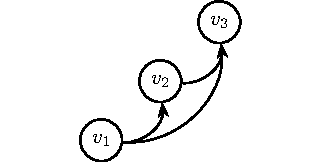
\includegraphics[width=1\linewidth]{figuras/graph2.pdf}
            \caption{Grafo original}
            \label{graph2}
        \end{subfigure}
        \begin{subfigure}[t]{0.49\textwidth}
            \centering
            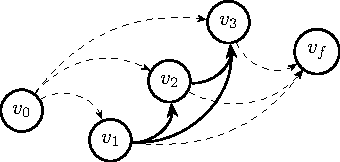
\includegraphics[width=1\linewidth]{figuras/graph3.pdf}
            \caption{Grafo com os nós fictícios}
            \label{graph2}
        \end{subfigure}
        \caption{Grafo com e sem nós fictícios}
    \end{figure}
\end{frame}

\section{Proposta}
\begin{frame}
    \frametitle{Proposta}
    \begin{itemize}
        \item Encorporar o uso de (meta) heurísticas na solução do subproblema;
        \item Segundo~\ccite{dos2008metodo} a utilização de meta heurísticas pode acelerar o processo de solução;
        \item Utilizar as heurísticas do subproblema para gerar um conjunto inicial de colunas;
    \end{itemize}
\end{frame}

\begin{frame}
    \frametitle{Proposta}
    {
        \centering
        \includegraphics[height=.8\textheight]{../tcc/figuras/flowchart.pdf}
        \captionof{figure}{Proposta de geração de colunas, adaptado de~\ccite{dos2008metodo}}
        \label{flowchart}
    }
\end{frame}

\begin{frame}
    \frametitle{(Meta) heurísticas estudadas}
    \begin{itemize}
        \item Busca gulosa baseada em relaxação linear;
        \item Subida de encosta;
        \item \textit{Simmulated annealing} (SA);
        \item \textit{Ant colony optimization} (ACO);
        \item Busca Tabu;
    \end{itemize}
\end{frame}

%\begin{frame}
    %\frametitle{Formulação do Subproblema}

%\end{frame}

\section{Conclusões parciais}
\begin{frame}
    \frametitle{Conclusões parciais}
    \begin{itemize}
        \item Pode-se identificar um problema teórico e com interesse prático;
        \item Realizou-se uma revisão bibliográfica onde:
        \begin{itemize}
            \item Identificou-se um método de solução para o problema;
            \item Identificou-se possíveis métodos para melhorar o desempenho do algoritmo;
        \end{itemize}
    \item Identificou-se um solver (\textbf{CPLEX}, GLKP, SCIP, Cbc, $\ldots$) para utilizar na solução do problema mestre
        e subproblema;
    \item Implementou-se um protótipo de geração de colunas capaz de resolver o CSP de forma exata;
    \end{itemize}
\end{frame}

\begin{frame}
    \frametitle{Próximas etapas}
    \begin{itemize}
        \item Seleção, implementação e avaliação das (meta) heurísticas para aplicar no subproblema;
        \item Utilização do banco de dados da \textit{OR-Libary} para avaliar a implementação final;
        \item Escrita do TCC-\RNum{2};
    \end{itemize}
\end{frame}

\begin{frame}
    \frametitle{Publicações}
    \begin{itemize}
        \item Artigo publicado na SBPO \RNum{48};
        \item Escrita de um artigo contemplando os resultados deste trabalho;
    \end{itemize}
\end{frame}

\begin{frame}
    \frametitle{Cronograma}
    \begin{center}
    \tiny
    \begin{tabular}{|c||c|c|c|c|c||c|c|c|c|c|c|}
        \hline
        \multirow{2}{*}{\textbf{{Etapas}}} & \multicolumn{5}{|c||}{\textbf{{2016}}} & \multicolumn{6}{|c|}{\textbf{{2017}}} \\
        \cline{2-12}
        & \textbf{A} & \textbf{S} & \textbf{O} & \textbf{N} & \textbf{D} & \textbf{J} & \textbf{F} & \textbf{M} & \textbf{A} & \textbf{M} & \textbf{J} \\
        \hline \hline
        \textbf{1} & \cellcolor{gray!50}\checkmark & \cellcolor{gray!50}\checkmark & \cellcolor{gray!50}\checkmark &                               &                               &                               &                               &                               &            &            & \\ \hline
        \textbf{2} &                               & \cellcolor{gray!50}\checkmark & \cellcolor{gray!50}\checkmark & \cellcolor{gray!50}\checkmark &                               &                               &                               &                               &            &            & \\ \hline
        \textbf{3} &                               & \cellcolor{gray!50}\checkmark & \cellcolor{gray!50}\checkmark & \cellcolor{gray!50}\checkmark & \cellcolor{gray!50}\checkmark &                               &                               &                               &            &            & \\ \hline
        \textbf{4} &                               & \cellcolor{gray!50}\checkmark & \cellcolor{gray!50}\checkmark & \cellcolor{gray!50}\checkmark & \cellcolor{gray!50}\checkmark &                               &                               &                               &            &            & \\ \hline
        \textbf{5} &                               &                               & \cellcolor{gray!50}\checkmark & \cellcolor{gray!50}\checkmark & \cellcolor{gray!50}\checkmark &                               &                               &                               &            &            & \\ \hline
        \textbf{6} &                               &                               &                               &                               &                               & \cellcolor{gray!50}\checkmark & \cellcolor{gray!50}\checkmark & \cellcolor{gray!50}\checkmark & \checkmark &            & \\ \hline
        \textbf{7} &                               &                               &                               &                               &                               &                               & \checkmark                    & \checkmark                    & \checkmark & \checkmark & \checkmark \\ \hline
        \textbf{8} &                               &                               &                               &                               &                               &                               &                               & \checkmark                    & \checkmark & \checkmark & \checkmark \\ \hline
        \textbf{9} &                               &                               &                               & \cellcolor{gray!50}\checkmark & \cellcolor{gray!50}\checkmark & \checkmark                    & \checkmark                    & \checkmark                    & \checkmark & \checkmark & \checkmark \\ \hline
    \end{tabular}
    \captionof{table}{Cronograma proposto com atividades completas em destaque}
    \end{center}
\end{frame}

%\section{Referências}

\begin{frame}
    %\bibliography{bibliografia}
    \printbibliography
\end{frame}

\end{document}
